\documentclass[margin=0mm,class=tufte-book]{standalone}
\usepackage{tikz}
\usepackage{pgfplots}
 \pgfplotsset{compat=newest}


\usepackage{amssymb,amsmath}

\usepackage[T1]{fontenc}
\usepackage[utf8]{inputenc}



\input{tint_book_header}



\begin{document}


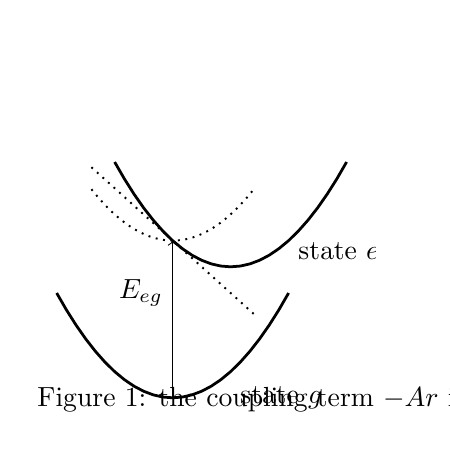
\begin{tikzpicture}
\useasboundingbox (0,0) rectangle (5,5);
%\draw (0,0) rectangle (6,6);

\begin{axis}[no markers, 
        domain=-1:1.5,
         axis y line=none,
           axis x line=none,
           width= 6cm]
\addplot [domain=-1:1,  line width=1pt]    {x^2};
\addplot  [domain=-0.5:1.5, line width=1pt]    {x^2 + 1.5 - x};

\addplot  [dotted, domain=-0.7:0.7, line width=0.7pt] {1.5 - x};
\addplot  [dotted, domain=-0.7:0.7, line width=0.7pt] {1.5 + x^2};

\addplot[->] coordinates
           {(0,0) (0, 1.5)};

\node[anchor=east] at (axis cs: 0,1) {$E_{eg}$};
\node[anchor= west] at (axis cs: 0.5,0) {state $g$};
\node[anchor=west] at (axis cs: 1,1.4) {state $e$};
           
\end{axis}

\node[above right] at (0,0) {Figure 1: the coupling term $- A r$ in the};

\end{tikzpicture}


\end{document}